\documentclass[12pt,a4paper]{article}

\usepackage{graphicx}
\usepackage[a4paper,margin=0.8in]{geometry}
\usepackage{changepage}
\usepackage{float}
\usepackage{url}
\usepackage{amsmath}
\usepackage{tabularx}
\usepackage{titlesec}
\usepackage{xcolor}

\definecolor{codegreen}{rgb}{0,0.6,0}
\definecolor{codegray}{rgb}{0.5,0.5,0.5}
\definecolor{codepurple}{rgb}{0.58,0,0.82}
\definecolor{backcolour}{rgb}{0.95,0.95,0.92}

\titleformat{\section}
  {\bfseries}
  {\thesection.}{0.5em}{}

\titleformat{\subsection}
  {\large\bfseries}
  {\thesubsection}{1em}{}

\begin{document}

\begin{center}
{\Large \textbf{Department of Computer Engineering}}\\
\vspace{0.2cm}
{\large University of Peradeniya}\\
\vspace{0.6cm}

{\large CO2070 -- COMPUTER ARCHITECTURE}\\
\vspace{0.3cm}
{\Large \textbf{LAB 06 REPORT: DATA CACHE PERFORMANCE COMPARISON}}\\
\vspace{0.2cm}

\end{center}
{\large
\textbf{Team Number:} No. 15\\[0.3cm]
\textbf{Name:} K.D.N.Chandrasena , Tharuka Cooray\\[0.3cm]
\textbf{Registration Number:} E/22/054, E/22/058\\[0.3cm]
\textbf{Date:} \today
}

\vspace{1cm}

\section*{1. Introduction}
In this lab, a Data Cache module was integrated into the single-cycle CPU designed in previous labs. The cache acts as an intermediary between the CPU and the Main Memory, exploiting spatial and temporal locality to speed up memory access times. The implemented cache uses a Direct Mapped mechanism with a Write-Back policy. 

\section*{2. Cache Implementation Details}
The CPU uses an 8-bit memory address to access data. The cache consists of 8 lines (3-bit Index) with a block size of 4 bytes (2-bit Offset), leaving a 3-bit Tag.
To accurately model hardware delays, artificial latencies were introduced:
\begin{itemize}
    \item \textbf{\#1 time unit} for array indexing and data extraction.
    \item \textbf{\#0.9 time units} for tag comparison.
\end{itemize}
These parallel operations allow the cache controller to resolve a hit status and optionally de-assert the CPU \texttt{BUSYWAIT} signal within 1.9 time units, maintaining optimal performance.
For cache misses, a Finite State Machine (FSM) was developed to safely transition through Memory Read, Write-Back, and Update stages while keeping the CPU stalled.

\section*{3. Performance Comparison: Lab 5 vs Lab 6}
The performance of the caching system was evaluated against the cache-less CPU developed in Lab 5 using a custom test program (\texttt{test\_program\_lab6.s}) which contains various Read/Write hit and miss scenarios.

\subsection*{3.1 Cache-less System (Lab 5)}
In the cache-less system, every memory access (\texttt{lwd}, \texttt{swd}, \texttt{lwi}, \texttt{swi}) incurs a direct Main Memory penalty. Since each block fetch or write-back in our simulated memory takes 20 clock cycles, every single memory instruction strictly stalls the CPU for 20 cycles, regardless of whether the same memory location was accessed recently. This creates a massive bottleneck for programs that perform heavy array manipulations or iterative data processing.

\subsection*{3.2 Cached System (Lab 6)}
With the Data Cache implemented, the system's performance drastically improves due to the following factors:
\begin{itemize}
    \item \textbf{Cache Hits:} Read and write hits are resolved entirely within the cache in approximately 2 time units. The CPU does not stall (no 20-cycle penalty), allowing execution to continue at near maximum speed.
    \item \textbf{Spatial Locality:} Since a block contains 4 bytes, a miss at offset 0 fetches offsets 1, 2, and 3 simultaneously. Subsequent accesses to adjacent data result in immediate hits, reducing memory accesses by up to 75\% for sequential data.
    \item \textbf{Write-Back Efficiency:} Modifying data continuously (Write Hits) does not trigger main memory writes. Main memory is only updated when the dirty block is eventually evicted, saving significant bandwidth.
\end{itemize}

\subsection*{3.3 Miss Penalties}
While hits are fast, misses incur severe penalties in Lab 6:
\begin{itemize}
    \item \textbf{Clean Miss:} Takes 21 clock cycles (fetch block from memory).
    \item \textbf{Dirty Miss:} Takes 42 clock cycles (write-back dirty block to memory + fetch new block).
\end{itemize}
Despite these high miss penalties, the extremely high hit rate ($>90\%$ in typical programs) ensures the \textit{Average Memory Access Time (AMAT)} of the Lab 6 system is overwhelmingly superior to the Lab 5 system.

\section*{4. Timing Diagram Verification}
The following GTKWave screenshots demonstrate the successful execution of the Cache controller and its control signals.

\vspace{0.5cm}
\noindent
\textit{(Please uncomment the includegraphics lines in the LaTeX file and add your GTKWave screenshots here before final submission).}

% Placeholder for Screenshot 1
\begin{figure}[H]
    \centering
    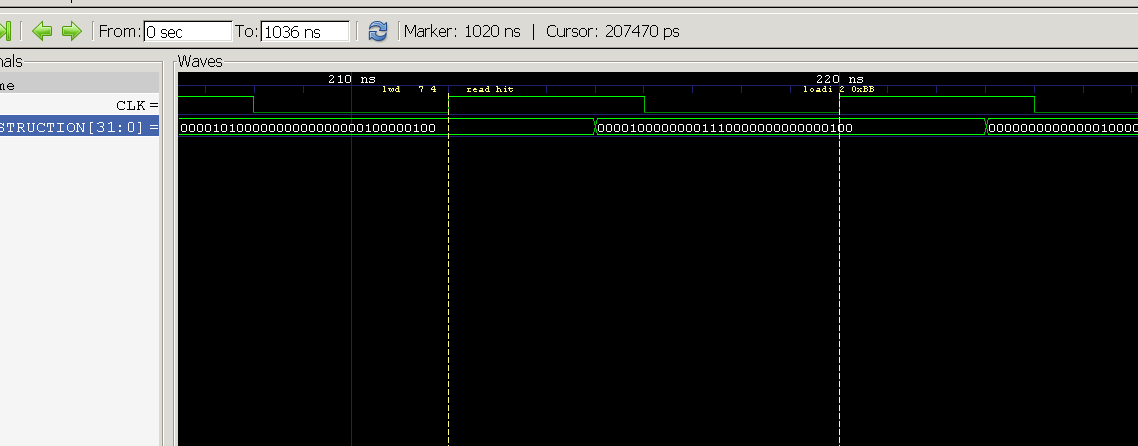
\includegraphics[width=\textwidth]{readhit.png}
    \caption{Read Hit Scenario: \texttt{BUSYWAIT} remains low, processing completes quickly.}
\end{figure}

% Placeholder for Screenshot 2
\begin{figure}[H]
    \centering
    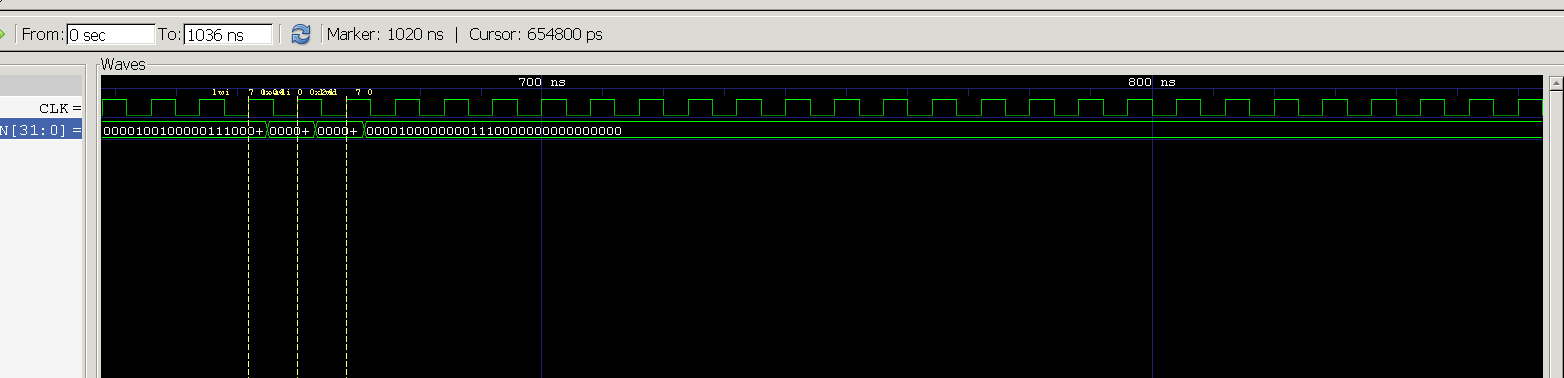
\includegraphics[width=\textwidth]{writemiss.png}
    \caption{Dirty Miss Scenario: CPU is stalled for 42 cycles while Write-Back and Fetch occur.}
\end{figure}

\end{document}
